\if 0
\begin{figure*}[ht]
    \centering
    \subfigure[Network Scan (Timeline)] {
        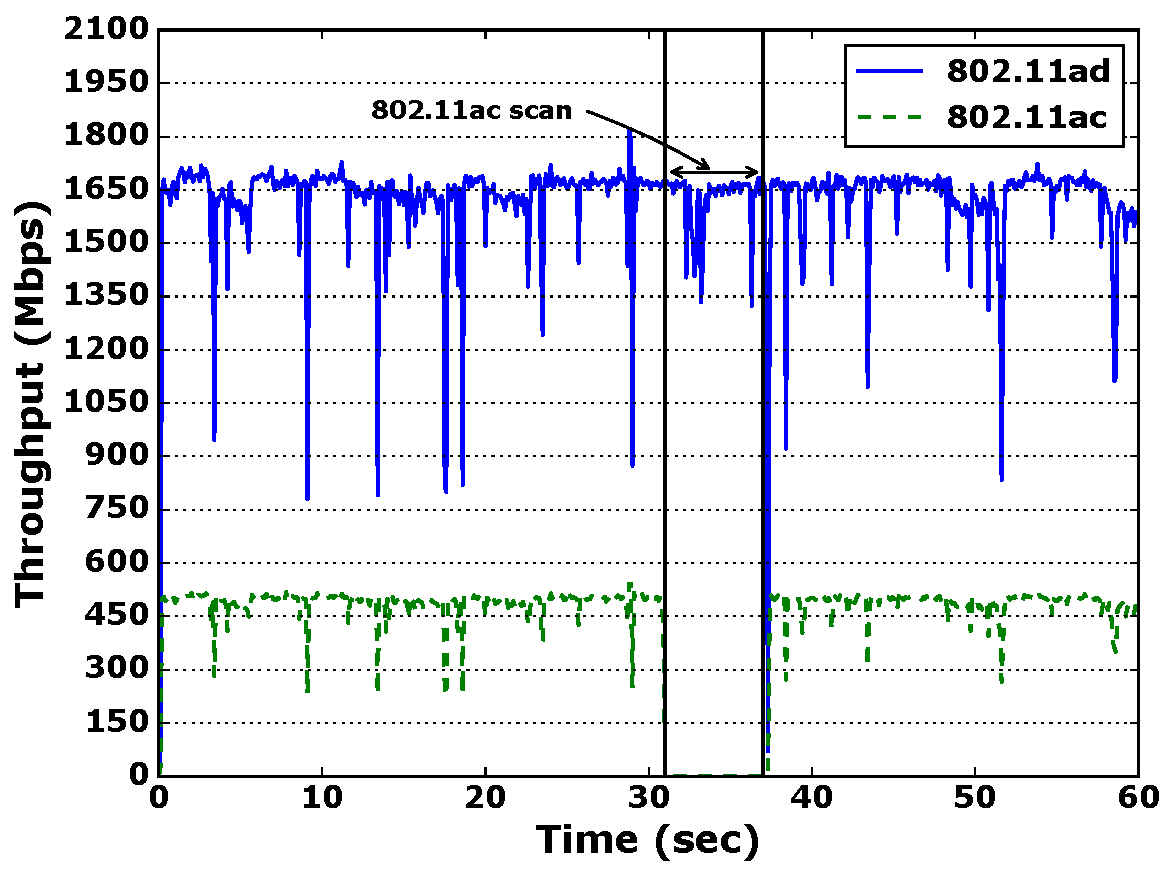
\includegraphics[scale=0.27]{NetworkManagerScan/timeline_fix.pdf}
        \label{fig:scan_fixed}
    }\hfill
    \subfigure[\emph{minRTT} vs. \emph{FixedRatio}] {
        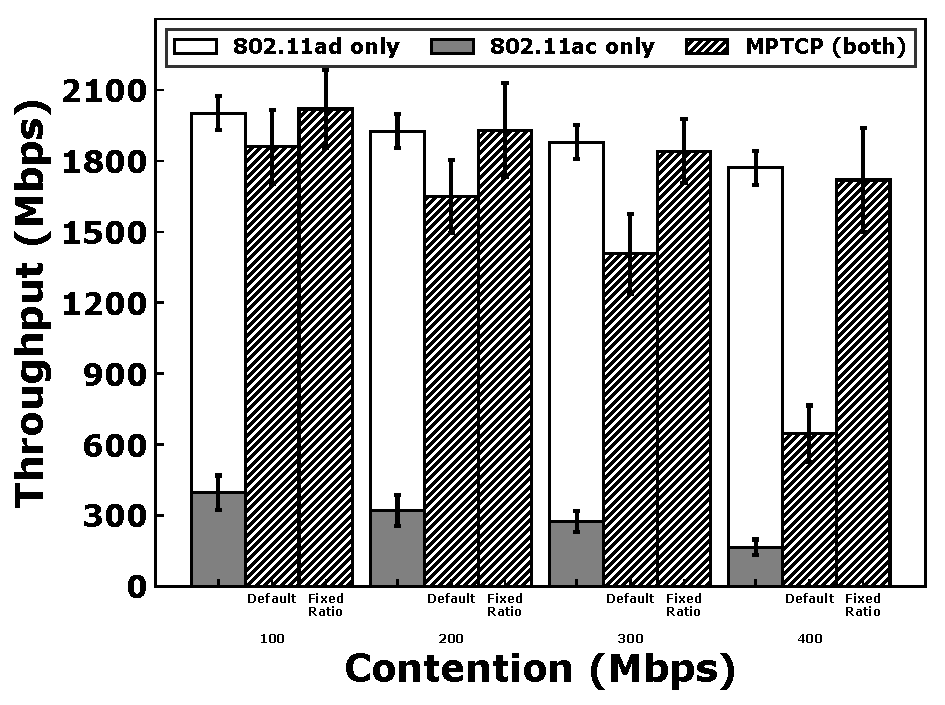
\includegraphics[scale=0.34]{contention/barplot.pdf}
        \label{fig:contention_barplot}
    }\hfill
    \subfigure[802.11ad Blockage: Improved recovery time] {
        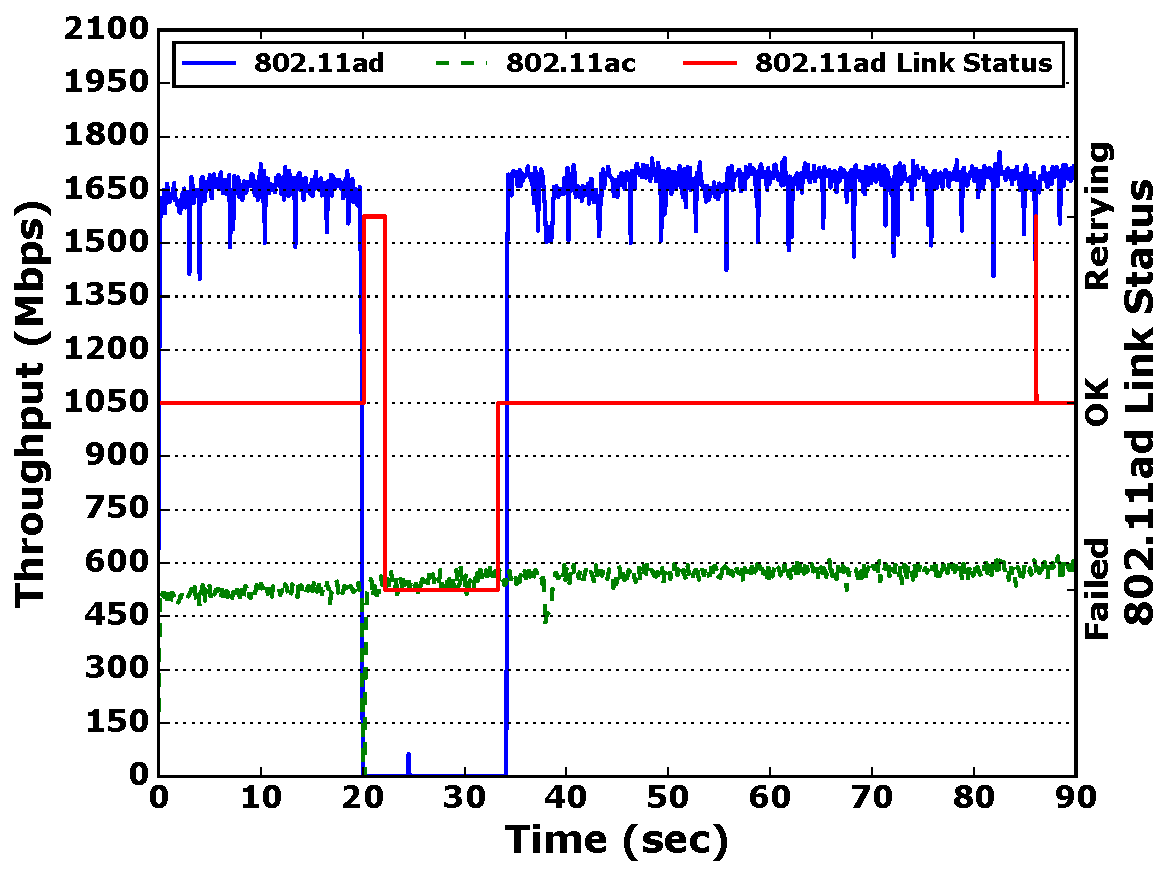
\includegraphics[scale=0.27]{blockage/blockage_fixed.pdf}
        \label{fig:blockage_recovery}
    }
    \vspace{-0.15in}
    \caption{\name}
    \vspace{-0.1in}
\end{figure*}
\fi

\noindent\textbf{\name-SCAN} arbitrates the network scan requests generated
from the user space and disables the scheduling of packets to the
subflow where the request has been made for the duration of the
network scan. However, disabling future scheduling alone may not be
enough to prevent packets from being held-up in the TCP queues or at
any of the buffers in the lower layers of the network stack. We thus
adopt a two-step approach, where \name: (1) stops the assignment of
packets to subflow about to undertake scanning and (2) waits for the
subflow-level \emph{send-queue} to be emptied out. Fig.~\ref{fig:scan_fixed} shows 
a timeline consisting of 802.11ac scan (marked as "802.11ac scan") but with \name's 
network scan management solution applied during the scan period. We can clearly see (compared
to the scan period in Fig.~\ref{fig:scan_issue}) that the 802.11ad
throughput remains unaffected during the scan interval. We repeat the
measurements several times with and without \name-SCAN fix and found 
that on average it improves from 700 Mbps to 1650 Mbps (\textbf{2.2x} gain).
\\
\noindent\textbf{\name-CONTENTION} leverages our findings regarding the 
existence of a unique MPTCP throughput-optimal ratio, given subflow throughput values. The 
reaction to contention on 802.11ac is to set the packet-assignment ratio to match the ratio of
the throughput of 802.11ad and 802.11ac flows, accounting for the drop
in 802.11ac throughput due to contention. We test our proposed
solution under different amounts of contention varying from 100 Mbps
to 400 Mbps. Fig.~\ref{fig:contention_barplot} shows the expected sum,
after accounting for 802.11ac throughput reduction in the presence of
contention, and MPTCP performance under the default
and \emph{FixedRatio} scheduler, which uses the optimal ratio for a
given amount of contention. In all cases, the default scheduler
achieves less than the expected sum with the magnitude of gap
increasing with contention.
\\
\noindent\textbf{\name-BLOCKAGE} reduces the delay in resuming traffic over the 802.11ad
subflow by resetting the {{\tt pf}} flag to allow for traffic to be
scheduled on the 802.11ad subflow. However, we found that this alone
was not enough to resume the traffic flow on the 802.11ad
interface. When the 802.11ad link is blocked, the
subflow-level \emph{cwnd} is cut to 1, with packets in flight also
equal to one. As a result, the scheduler is unable to schedule any new
packets on 802.11ad subflow as the \emph{cwnd} is reported as being
full. In order to overcome this, \name uses the TCP's window recovery
mechanism to restore the \emph{cwnd} to the value just before loss the
event. In contrast to Fig.~\ref{fig:blockage_tput_drop}, where MPTCP resumed traffic on the
802.11ad subflow after a 20 s delay, with \name engaged (fig. \ref{fig:blockage_recovery}) 
MPTCP starts using the 802.11ad interface in less than 1s after link re-establishment. This
is a vast reduction in delay for resuming traffic on the subflow. In a
dynamic environment, where such blockage events will occur quite
frequently, \name's gains would translate into a significant
improvement in user-experience.
